\chapter{Evaluation}

\section{Introduction}

In this chapter, we investigate the performance characteristics of the two runtimes we created for FrDataFlow. We will explore different types of reactive programs and how they behave under high loads of data, comparing them on a few metrics. More specifically, we will focus on the following metrics:

\begin{description}[style=nextline]
  \item [Latency]		The time it takes for a value to propagate through the entire graph of signals
  \item [Throughput]	The amount of values that can propagate through the entire graph within a certain time frame.
  \item [Scaling]		The amount of performance that can be gained by executing the program in parallel
\end{description}

\section{Topologies}

Before we can start running benchmarks, we must first define the types of programs that we are interested in profiling. In \textit{Optimizing Distributed REScala} \cite{drechsler_optimizing_2014}, three topologies are suggested that sufficiently represent any reactive program for the purposes of evaluating performance.

\subsection{Linear}

This model is the simplest one: we have a graph of signals where each signal only has one parent and one child. When the source signal emits a new value, it simply propagates through the graph in one linear motion and stops at the end. 

\begin{figure}[h]
	\centerline{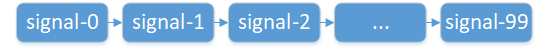
\includegraphics[scale=0.7]{images/Evaluation-Topologies-Linear.png}}
	\caption{A linear topology: each signal has one parent and one child}
	\label{fig:evaluation-topologies-linear}
\end{figure}

\subsection{Fan out}

In this topology, our graph immediately splits up into many children, as shown in figure \ref{fig:evaluation-topologies-fanout}. This is a scenario where one source signal provides important data that every other signal depends upon. The interesting effect of this is when that specific source signal emits a new value, it will trigger an immediate high load of updates for all of its children. 

\begin{figure}[h]
	\centerline{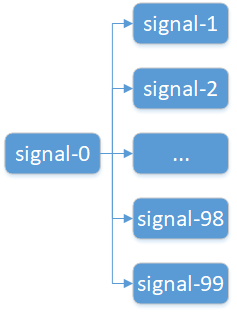
\includegraphics[scale=0.7]{images/Evaluation-Topologies-Fanout.png}}
	\caption{A fan-out topology: one signal with a large amount of children}
	\label{fig:evaluation-topologies-fanout}
\end{figure}

\subsection{Square}

The square topology is expected to be the most common, it provides a signal graph that is not extremely deep such as the linear topology nor is it very wide like the fan-out variant. In this topology, signals have a variable amount of parents and children, shaping the graph into a square. For the purposes of our benchmarks, we will use an exact square graph for simplicity.  

\begin{figure}[h]
	\centerline{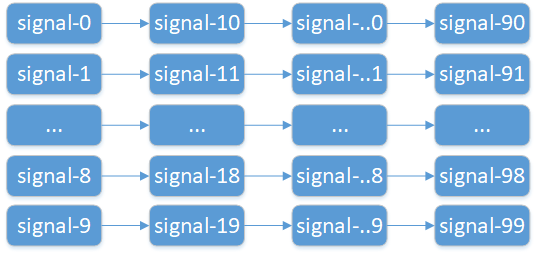
\includegraphics[scale=0.7]{images/Evaluation-Topologies-Square.png}}
	\caption{A square topology: The signal graph is equally deep as it is wide}
	\label{fig:evaluation-topologies-square}
\end{figure}

\section{Benchmarks}

All of the benchmarks in this chapter are run in the Racket VM with unlimited memory (16 GB RAM physical limit) and on an AMD Phenom II X4 955 processor (Quad core, 3.2 GHz). Three sample programs were created with around 100 signals each, each of which implementing one of the three topologies as shown in the diagrams. These programs were each executed three times for 60 seconds, taking the averages of the output to produce the charts in this chapter.
A single source signal was emulated to emit 10 million values per second and the output nodes of the signal graphs were inspected to collect information on how many values were propagated through the graph and at what rate the update mechanisms could keep up with the stream of incoming data. 

\newpage
\subsection{Without dataflow engine}

We will first evaluate the runtime that implements an update loop in the interpreter itself and does not use the dataflow model to keep its graphs up to date. These are the tests for our first runtime for FrDataFlow. 

\subsubsection{Latency}

\begin{figure}[h]
	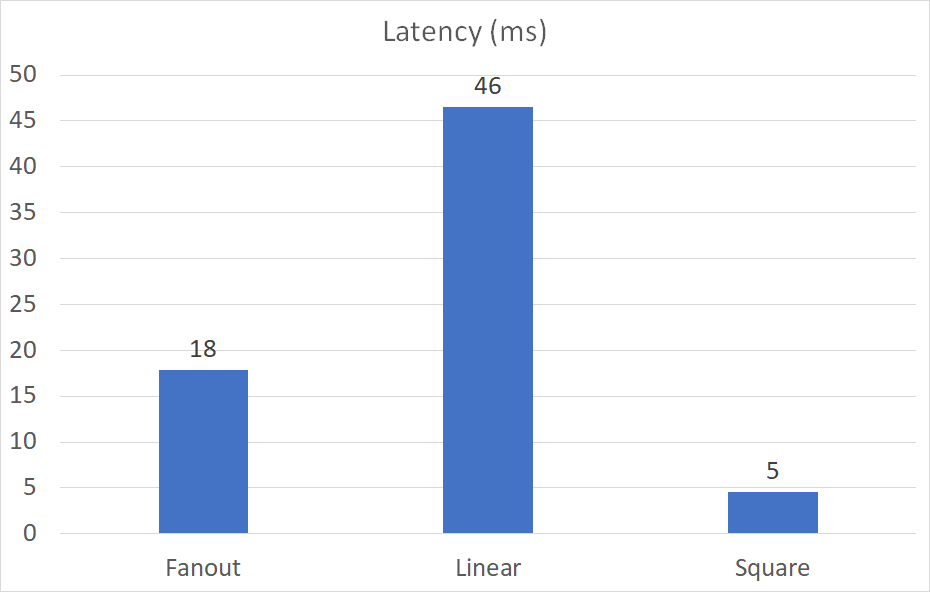
\includegraphics[width=\textwidth]{images/Evaluation-WithoutDataFlow-Latency.png}
	\caption{The latency of signals in FrDataFlow without the dataflow engine}
	\label{fig:evaluation-withoutdataflow-latency}
\end{figure}

Inspecting these results, we conclude that the linear graph show the highest latency, which is expectable: values in this topology travel the longest path of signals before they reach the end. On average, it took nearly 50 ms for a value to propagate from the source signal to the last output node.
More interestingly, values in the fanout topology seem to take longer on average to reach the end than in the square variant. This is counterintuitive, because every value in the fanout graph only needs to pass two signal nodes before it reaches the end. Since the fanout graph contains 99 output nodes and the square graph only 10, it would seem that this gives the square graph a slight edge: these 10 output nodes have to wait less long to be given the chance to announce their output. 

\subsubsection{Throughput}

\begin{figure}[h]
	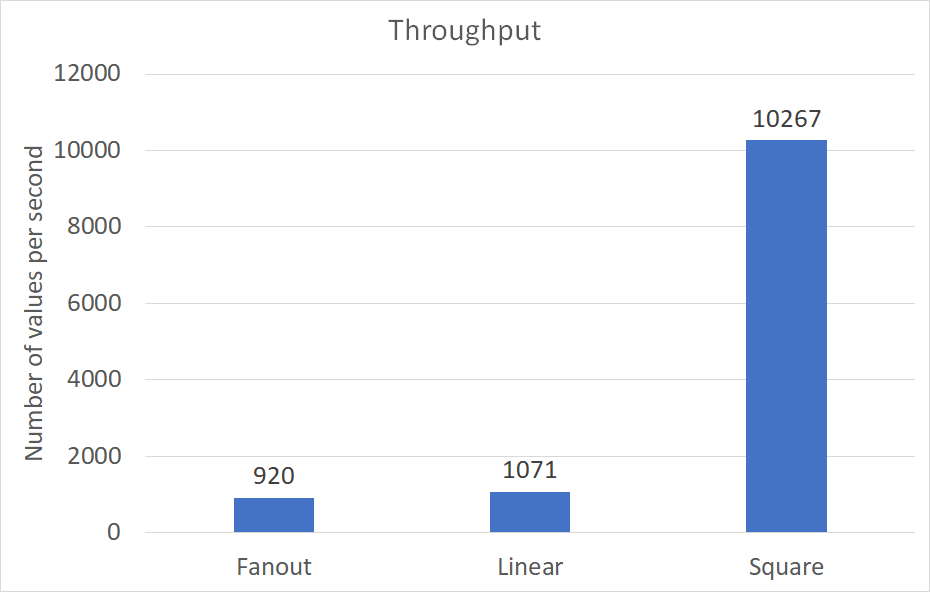
\includegraphics[width=\textwidth]{images/Evaluation-WithoutDataFlow-Throughput.png}
	\caption{The throughput of signals in FrDataFlow without the dataflow engine}
	\label{fig:evaluation-withoutdataflow-throughput}
\end{figure}

Even more so than with latency, the square topology is the clear winner when it comes to the sheer amount of values it can push through the graph per second. The square graph can push out more than 10 000 values per second and is an order of magnitude more efficient compared to the fanout or linear approach, who only managed to process 1 000 values by and large. This makes sense, because every update loop iterates over all the signal nodes once. In the square topology, this means it can propagate 10 values to the end in one loop. The linear version on the other hand can only process one, because when the iteration is happening it is really pushing forward one value from the first signal all the way to the last. Similarly, the fanout approach results in one loop pushing a single value from the first signal to all other signals. The square topology, by splitting up the graph in 10 linear parts, essentially 
parallelizes this work. 

\newpage
\subsection{With dataflow engine, single core}

In this section, we repeat the same tests of the previous section but this time using the runtime that sits atop the dataflow engine. The programs are exactly the same, but they are now compiled to dataflow instructions and invoked there. These are the tests for our second runtime for FrDataFlow. 

\subsubsection{Latency}

\begin{figure}[h]
    \includegraphics[width=\textwidth]{images/Evaluation-WithDataFlow-Latency.png}
	\caption{The latency of signals in FrDataFlow with the dataflow engine}
	\label{fig:evaluation-withdataflow-latency}
\end{figure}

The first thing that is immediately obvious is the general increase in latency, except for the linear topology. We observe an average of 50 ms extra latency because we now translate to dataflow instructions. This was to be expected: the use of a dataflow engine brings with it some extra overhead such as the management of the token queue. While 50 ms is considerable, it is not a show stopping performance penalty and is thus acceptable for the gains that can be made in other spaces. Special mention goes to the linear topology, which seems the only approach to actually decrease the average latency. The dataflow engine seems optimized for a linear cascading chain of tokens when it comes to latency.

\subsubsection{Throughput}

\begin{figure}[h]
	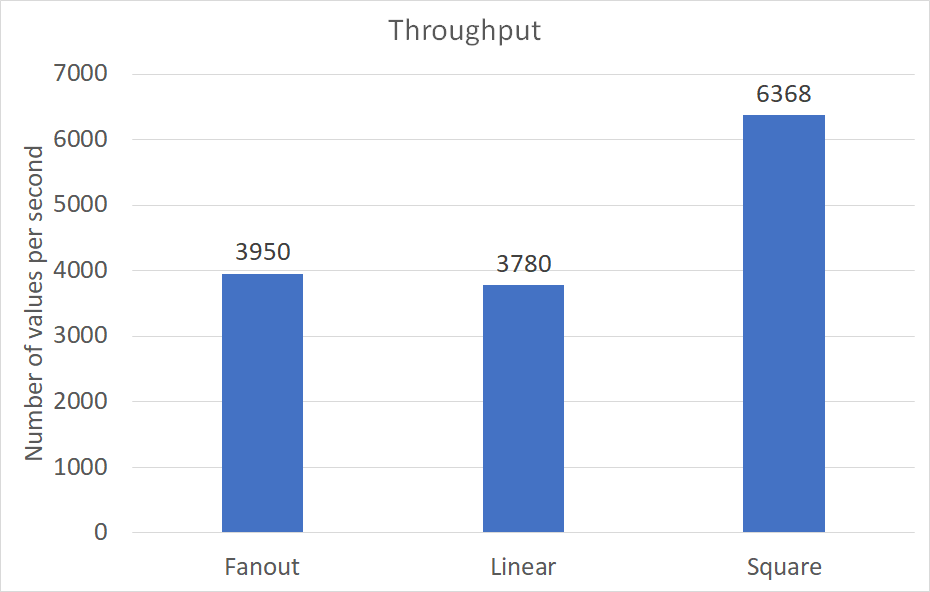
\includegraphics[width=\textwidth]{images/Evaluation-WithDataFlow-Throughput.png}
	\caption{The throughput of signals in FrDataFlow with the dataflow engine}
	\label{fig:evaluation-withdataflow-throughput}
\end{figure}

We observe that the general throughput using the dataflow engine is more efficient than the first runtime. 
Especially the fanout and linear approaches benefit here and see a tripling of their output. The square topology on the other hand is less advantaged by the second runtime and takes a small hit in throughput compared to the first runtime.

The major reason for this increase in throughput can be attributed to the compilation step of the signals that happens in the mapping algorithm. In the first runtime, the update lambdas associated with each signal are fed into the metacircular evaluator which has to lookup variables in the lexical scope and generally introduces a significant overhead just to call a lambda and pass on a value. When running atop the dataflow engine, these update lambdas are fed natively to the dataflow engine which has no knowledge of the metacircular evaluator, which allows it to skip most of the evaluation steps that are necessary in the first runtime.

The reason why the square topology does a little worse is because the update loop in the first runtime is - by accident - ideally optimized for square topologies, while the dataflow engine is not: tokens are just processed one by one, which levels the playing field for all three topologies. 

\subsection{With parallelization, four cores}

In this section, we repeat the same tests a third time but this time configuring the dataflow engine to spread its work across 4 cores. The engine does this by making use of Racket Places \cite{tew_places:_2011}, which starts up a configurable amount of runtimes. 

\subsubsection{Latency}

\begin{figure}[h]
	\includegraphics[width=\textwidth]{images/Evaluation-WithDataFlowParallel-Latency.png}
	\caption{The latency of signals in FrDataFlow with the dataflow engine running on four cores}
	\label{fig:evaluation-withdataflow-latency}
\end{figure}

By switching to four different processor cores, the fanout topology was most negatively impacted. By distributing the queue of token across four different instances, tokens took nearly a second each to reach their destination. 
The linear approach on the other hand strongly benefits from the parallelisation: we see that each chain of values that travels to the end of the graph is still extremely fast. Latency wise, there was no penalty for the linear and square topology, resulting in a net loss of throughput.

\subsubsection{Throughput}

Even though the latency of the fanout approach is quite worse than its non parallel alternative, it did positively impact the throughput of this topology. Since this approach results in immediate bursts of new tokens, the fact that four processes are simultaneously picking these tokens up gives it an edge over the other topologies. 
Surprisingly, the square topology suffers most from the split up into multiple parallel instances of the dataflow engine. It seems that the communication between the instances causes more overhead in this topology than the benefits of distributing the work. Racket channels seem to cause a lot of delay to get values to the end of the graph. 

\begin{figure}[ht]
	\includegraphics[width=\textwidth]{images/Evaluation-WithDataFlowParallel-Throughput.png}
	\caption{The throughput of signals in FrDataFlow with the dataflow engine running on four cores}
	\label{fig:evaluation-withdataflow-throughput}
\end{figure}

\subsection{Discussion of results}

From the results of our benchmarks, we can first conclude that latency generally increases when running atop the dataflow engine, especially when running it in parallel is added to the equation. This was to be expected: the dataflow execution model goes through more phases and needs more bookkeeping than the update loop of the first runtime to support the same behavior. On the other hand, it provides more scalability. We see that the throughput globally increases when running atop the dataflow engine, although the introduction of parallelism does not result in better throughput. We attribute this to two characteristics of our implementation:

\begin{enumerate}
	\item Racket places communicate across threads using channels, which does not come cheaply. This communication overhead, with certain topologies, unfortunately is more detrimental for the throughput than the benefits it brings. 
	\item In our benchmarks, the signal update callbacks merely pass on incoming values rather than doing a meaningful computation. While this is common in reactive programming, it does mean that calling these callbacks is extremely fast and that parallelizing them will only be beneficial if the overhead of parallelisation is negligible. 
\end{enumerate}

\section{Conclusion}

In this chapter we presented numbers that show the performance of three sample programs that implement different topologies. We tested these programs using a simple update loop in the first runtime, using the dataflow engine on a single processor and using the dataflow engine on four processor cores. Collecting these results, we conclude that while the signs of scalability are there, in our current setup the benefits are not visible. As long as the overhead of running in parallel is not reduced to the bare minimum, it will require large signal graphs and a large amount of parallellism to be more efficient than simple single threaded approaches in terms of latency and throughput. In our implementation, this overhead is still too considerable to make the effort worthwhile. 



